\documentclass[25pt]{article}
\usepackage[a4paper, top=3cm, left=3cm, right=2.5cm, bottom=2.5cm]{geometry}
\usepackage{lmodern}
\usepackage[T1]{fontenc}
\usepackage[portuges]{babel}
\usepackage[utf8]{inputenc}
\usepackage{a4}
\usepackage[document]{ragged2e}
\usepackage{textgreek}
\usepackage{epstopdf}
\usepackage{graphicx}
\usepackage{fancyvrb}
\usepackage{amsmath}
\usepackage{float}
\usepackage{listings}


\begin{document}

\begin{titlepage}

\newcommand{\HRule}{\rule{\linewidth}{0.5mm}} % Defines a new command for the horizontal lines, change thickness here

\center % Center everything on the page

%----------------------------------------------------------------------------------------
%	HEADING SECTIONS
%----------------------------------------------------------------------------------------

\textsc{\LARGE Universidade do Minho}\\[1.5cm]
\HRule \\[0.4cm]
{ \huge \bfseries Programação em Lógica Estendida e Conhecimento Imperfeito}\\[0.4cm]
\HRule \\[1.5cm]
\textsc{\Large Mestrado Integrado em Engenharia Informática}\\[0.5cm]
\textsc{\large Sistemas de Representação de Conhecimento e Raciocínio}\\[0.5cm]
\textsc{\large 2ºSemestre 2018/19}\\[0.5cm]


%----------------------------------------------------------------------------------------
%	AUTHOR SECTION
%----------------------------------------------------------------------------------------

\begin{minipage}{0.4\textwidth}
\begin{flushleft} \large
\emph{Grupo:}\\
Etienne Costa A76089 \\
Joana Cruz A76270 \\
Rui Azevedo A80789 \\
Maurício Salgado A71407 \\
João Coutinho A86272 \\
\end{flushleft}
\end{minipage}
~
\begin{minipage}{0.4\textwidth}
\begin{flushright} \large
\emph{Docente:} \\
César Analide\\
\end{flushright}
\end{minipage}\\[2cm]

%----------------------------------------------------------------------------------------
%	DATE SECTION
%----------------------------------------------------------------------------------------

{\large \today}\\[2cm]

%----------------------------------------------------------------------------------------
%	LOGO SECTION
%----------------------------------------------------------------------------------------

% 
\includegraphics[scale=0.3]{uminho}\\

%----------------------------------------------------------------------------------------

\vfill % Fill the rest of the page with whitespace

\end{titlepage}



\newpage
\tableofcontents

\newpage
\section{Resumo}
 O presente trabalho tem como principal objetivo aprofundar os conhecimentos na linguagem de programação em lógica PROLOG.\newline
 Com base nisso foi desenvolvido o relatório explicando o desenvolvimento do segundo exercício prático no âmbito da unidade
 curricular de Sistemas de Representação de Conhecimento e Raciocínio.\newline
 Este trabalho desenvolvido consiste na implementação de um sistema de representação de conhecimento e raciocínio com capacidade
 para caracterizar um universo de discurso na área da prestação de cuidados de saúde tirando partido da programação em lógica estendida
e à representação de conhecimento imperfeito, recorrendo à temática dos valores nulos.\newline


\newpage
\section{Introdução}
O relatório apresentado diz respeito ao segundo exercício proposto no âmbito da unidade curricular de Sistemas de
Conhecimento de Representação e Raciocínio, utilizando a linguagem de programação em lógica PROLOG. O universo de discurso
para qual estamos a desenvolver este sistema é o universo de prestação de cuidados de saúde, assim esta base de conhecimento consiste
em utentes, serviços, consultas e prestadores de serviços.
\newpage

\section{Preliminares}
Para o desenvolvimento deste projeto foi necessário alguns conhecimentos previamente adquiridos de programação em lógica, e a
utilização da linguagem PROLOG. Este conhecimento foi absorvido durante as aulas de Sistemas de Representação de Conhecimento e Raciocínio,
e também com alguma pesquisa nossa. De seguida, apresentamos alguns conceitos fundamentais para a compreensão e realização deste trabalho.
\subsection{Programação em lógica e PROLOG}

Uma das principais ideias da programação em lógica é de que um algoritmo é constituído por dois
elementos disjuntos: a lógica e o controle. O componente lógico corresponde à definição do que deve
ser solucionado, enquanto que o componente de controle estabelece como a solução pode ser obtida.
O programador precisa somente descrever o componente lógico de um algoritmo, deixando o controle
da execução para ser exercido pelo sistema de programação em lógica utilizado. Em outras palavras, a
tarefa do programador passa a ser simplesmente a especificação do problema que deve ser solucionado, razão pela qual as
linguagens lógicas podem ser vistas simultaneamente como linguagens para
especificação formal e linguagens para a programação de computadores.
O paradigma fundamental da programação em lógica é o da programação declarativa, em oposição à
programação procedimental típica das linguagens convencionais.
Um programa em lógica é então a representação de determinado problema ou situação expressa através de um conjunto finito
de um tipo especial de sentenças lógicas denominadas cláusulas.
Pode-se então expressar conhecimento (programas e/ou dados) em Prolog por meio de cláusulas de
dois tipos: fatos e regras. Um fato denota uma verdade incondicional, enquanto que as regras definem as condições que devem ser satisfeitas para que
uma certa declaração seja considerada verdadeira. Como fatos e regras podem ser utilizados conjuntamente, nenhum componente
dedutivo adicional precisa ser utilizado. Além disso, como regras recursivas e não-determinismo são permitidos, os programadores podem obter
descrições muito claras, concisas e não-redundantes da informação que desejam representar. Como não há distinção entre argumentos
de entrada e de saída, qualquer combinação de argumentos pode ser empregada.
Os termos "programação em lógica" e "programação Prolog" tendem a ser empregados indistintamente. Deve-se, entretanto, destacar
que a linguagem Prolog é apenas uma particular abordagem da
programação em lógica.
\newpage

\section{Descrição do Trabalho e Análise dos Resultados}

De modo a complementar o sistema a ser desenvolvido foi implementado o conhecimento imperfeito e a lógica estendida, sendo assim
foi introduzido um valor de verdade novo,isto é, o desconhecido.
Para além disso , surge a possibilidade de representar conhecimento negativo,positivo e o imperfeito, sendo que este último pode ser
incerto,impreciso ou mesmo interdito. 
Foram construídas certas regras da negação dos predicados de modo que seja possível obter resposta mesmo quando não exista facto negativos e para
tal foi adotado o pressuposto do mundo fechado.




\section{Base de conhecimento}
Um programa em Prolog é um conjunto de axiomas e de regras de inferência definindo relações entre objectos que descrevem
um dado problema. A este conjunto chama-se normalmente base de conhecimento.\\
A base de conhecimento do sistema desenvolvido é essencial à representação do conhecimento e raciocínio,tendo em conta o sistema
foram desenvolvidas as seguintes entidades:

\begin{itemize}
  \item utente: \#IdUt, Nome, Idade,Sexo, Cidade $\to$ \{V,F\}
  \item serviço: \#IdServ,Especialidade,Instituiç\~ao,Cidade $\to$ \{V,F\}
  \item consulta:\#IdConsult,\#IdUt,\#IdPrestador,\#IdServ,Descrição,Custo,Data $\to$ \{V,F\}
  \item prestador:\#IdPrestador,\#IdServ,Nome,Idade,Sexo $\to$ \{V,F\}
  
  \end{itemize}



\subsection{Entidades}
Nesta secção são apresentadas e caraterizadas as Entidades acima propostas.

\subsubsection{Utente}
Num mundo real o utente é caracterizado por diversos factores , que por sua vez no contexto do Prolog esses factores passam a ser denomindados por átomos cujo o seu propósito é identifcar os objectos. Sendo assim para os utentes optou-se por usar os seguintes átomos:

 \begin{itemize}
  \item IdUt: Identificador do utente,que por sua vez é um valor único.
  \item Nome: Nome do utente.
  \item Idade: Idade do utente.
  \item Sexo: Sexo do utente.
  \item Cidade: Cidade aonde mora o utente.
\end{itemize}

\subsubsection{Serviço}
Um serviço por sua vez é  caracterizado pelos seguintes átomos:
\begin{itemize}
  \item IdServ: Identificador do serviço, que por sua vez é uma valor único.
  \item Especialidade: Referente ao serviço prestado.
  \item Instituição: Espaço físico aonde é efectuado o serviço.
  \item Cidade: Espaço geográfico aonde se encontra a instituição.
\end{itemize}

\subsubsection{Consulta}
Uma consulta será sempre referente a um utente, a um prestador de serviço e a um serviço, sendo que a mesma é realizada numa data específica e tem sempre uma breve descrição e custo associado , portanto optou-se por representar o conhecimento do seguinte modo:

\begin{itemize}
  \item IdConsult: Identificador da consulta, que por sua vez é uma valor único.
  \item IdUt: Identificador do utente.
  \item IdPrestador: Identificador do prestador de serviço.
  \item IdServ: Identificador do serviço prestado.
  \item Descrição:Breve descrição da consulta.
  \item Custo: Custo associado à consulta.
  \item Data: Data da realização da consulta.
\end{itemize}

\subsubsection{Prestador}
O prestador por sua vez é a entidade que presta os serviços existentes na base de conhecimento e para tal o mesmo é caracterizado pelos seguintes
átomos:

\begin{itemize}
  \item IdPrestador: Identificador do prestador, que por sua vez é uma valor único.
  \item IdServ: Identificador do serviço prestado.
  \item Nome:   Nome do prestador de serviço.
  \item Idade:  Idade do prestador.
  \item Sexo:   Sexo do prestador.
 \end{itemize}

\newpage


\section{Representação de Conhecimento}

Sendo que é necessário apresentar uma distinção entre o conhecimento positivio e negativo, surgiu
a necessidade de implementar o operador "-". Sendo que esse conhecimento negativo é representado por um negação
forte,isto é, informa que um dado termo é falso.\newline
Sendo assim eis à seguinte listagem das negações fortes implementadas :
\begin{lstlisting}

 -utente(IdUt,Nome,Idade,Sexo,Cidade):-
        nao(utente(IdUt,Nome,Idade,Sexo,Cidade)),
        nao(excecao(utente(IdUt,Nome,Idade,Sexo,Cidade))).


-servico(IdServ,Especialidade,Instituicao,Cidade):-
        nao(servico(IdServ,Especialidade,Instituicao,Cidade)),
        nao(excecao(servico(IdServ,Especialidade,Instituicao,Cidade))).

-consulta(IdConsult,IdUt,IdPrestador,IdServ,Descricao,Custo,Data):-
 nao(consulta(IdConsult,IdUt,IdPrestador,IdServ,Descricao,Custo,Data)),
 nao(excecao(consulta(IdConsult,IdUt,IdPrestador,IdServ,Descricao,Custo,Data))).


-prestador(IdPrestador,IdServ,Nome,Idade,Sexo):-
        nao(prestador(IdPrestador,IdServ,Nome,Idade,Sexo)),
        nao(excecao(prestador(IdPrestador,IdServ,Nome,Idade,Sexo))).

\end{lstlisting}

\subsection{Conhecimento positivo}

Quanto ao conhecimento posivito , este faz referência à informação existente na base de conhecimento.
Podemos interpretar o seguinte exemplo:
\begin{itemize}
\item utente(6,pedro,36,'M','Guimaraes').
\end{itemize}
 É verdadeiro que o Pedro é um utente que deu entrada no centro de saúde com o identificador igual à 6, e o mesmo reside em Guimarães
e possui o sexo masculino.

\begin{figure}[H]
\centering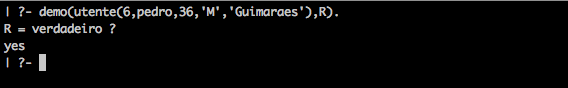
\includegraphics[scale=0.55]{positivo}
\caption{\label{fig:controller}Representação do conhecimento positivo.}
\end{figure}

\subsection{Conhecimento negativo}

Quanto ao conhecimento negativo, este faz referência à informação inexistente na base de conhecimento.
Podemos interpretar o seguinte exemplo:

\begin{itemize}
\item -utente(8,belo,45,'M','Dubai').
\end{itemize}

É falso que o Belo seja um utente que deu entrada no centro de saúde com o identificador igual à 8, que possua 45 anos e que reside na cidade
do Dubai possuindo o sexo masculino.

\begin{figure}[H]
\centering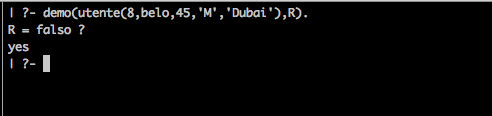
\includegraphics[scale=0.55]{negativo}
\caption{\label{fig:controller}Representação do conhecimento negativo.}
\end{figure}


\section{Conhecimento Imperfeito}

Nesta secção pretende-se fazer uma breve explicação e representação do tipo de valores mais comuns que podem surgir
numa situação de informação incompleta. Valores esses que são designados por valores nulo, sendo que os mesmos surgem como
uma estratégia para a enumeração de caso, para os quais se pretende fazer a distinção entre situações em que as respostas a questões
deverão ser concretizadas como verdadeiras,falsas ou desconhecidas.\newline
Serão três os valores nulos aqui representados:
\begin{itemize}
\item Incerto: Desconhecido, de um conjunto indeterminado de hipóteses.
\item Impreciso: Desconhecido, mas de um conjunto determinado de hipóteses.
\item Interdito: Desconhecido e não permitido conhecer.
\end{itemize}

\subsection{Incerto}
Para descrever um utente que tenha dado entrada em algum centro de saúde apesar do seu nome ser desconhecido adotou-se a seguinte representação:
\begin{lstlisting}
utente(11,name1,33,'F','Famalicao').
excecao(utente(IdUt,Nome,Idade,Sexo,Cidade)):- 
utente(IdUt,name1,Idade,Sexo,Cidade).
\end{lstlisting}

Utilizou-se o átomo name1 para representar o valor incerto relativo ao utente tirando partido da exceção do mesmo para representar o valor incerto.\newline
Como resposta ao exemplo apresentado obtemos a seguinte resposta:

\begin{figure}[H]
\centering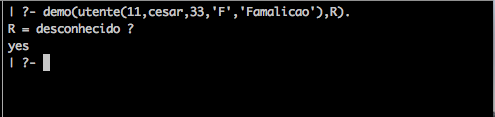
\includegraphics[scale=0.55]{incerto}
\caption{\label{fig:controller}Conhecimento Incerto de um Utente.}
\end{figure}

Dado que não existe conhecimento perfeito em relação ao utente acima mencionado , obtemos como esperado à resposta "desconhecido".


\subsection{Impreciso}
Como o próprio nome indica, este tipo de conhecimento posiciona-se em situações em que sabe-se que a informação é desconhecida mas pertence 
a uma gama de hipóteses. Esta imprecisão pode ser dividida em dois grupos:
\begin{itemize}
\item Conjunto de hipóteses distinguíveis.
\item Intervalo de valores.
\end{itemize}

Para o conjunto de hipóteses distinguíveis temos casos em que  o conhecimento representado é impreciso face aos valores que um determinado facto
apresenta.
Por exemplo temos a utente Marta de 55 anos cuja à sua morada é imprecisa pois não se sabe ao certo se a Marta reside em Guimarães ou Braga.

\begin{itemize}
\item excecao(utente(14,marta,55,'F','Guimaraes')).
\item excecao(utente(14,marta,55,'F','Braga')).
\end{itemize}

\begin{figure}[H]
\centering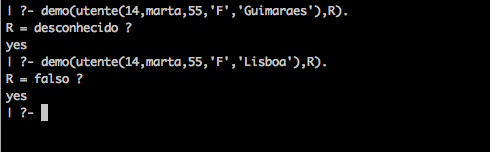
\includegraphics[scale=0.55]{impreciso1}
\caption{\label{fig:controller}Conhecimento Impreciso de um Utente.}
\end{figure}

Quanto ao intervalo de valores o exemplo mais prático seria a representação de um intervalo de idades, isto é, não ser preciso ao ponto 
de afirmar que o utente tem x anos de vida, mas sim que a sua idade esteja coomprendida num intervalo de valores.
Para tal temos o exemplo da Teresa que é uma senhora que reside na cidade de Paris, identificada pelo Id 13 mas a sua idade é imprecisa visto que
a idade da Teresa pertence ao intervalo [18,32].
\begin{itemize}
\item excecao(utente(13,teresa,Idade,'F','Paris')):- Idade>=18,
                        Idade=<32.
\end{itemize}

\begin{figure}[H]
\centering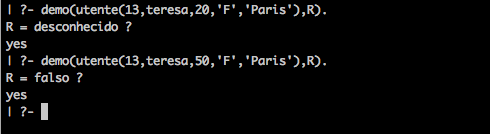
\includegraphics[scale=0.55]{impreciso2}
\caption{\label{fig:controller}Conhecimento Impreciso de um Utente.}
\end{figure}

\subsection{Interdito}
O conhecimento imperfeito do tipo interdito recai na situação em que o conhecimento relativo à uma entidade é desconhecido e permanecerá 
assim, não sendo possível saber o seu valor.\newline
Como exemplo temos o utente bernardo que por questões de confidencialidade não se sabe à sua cidade, sendo que este conhecimento é identificado
a custa do predicado nulo.

\begin{itemize}
\item nulo(interdito1).
\item utente(15,bernardo,24,'M',interdito1).
\item excecao(utente(IdUt,Nome,Idade,Sexo,Cidade)):- utente(IdUt,Nome,Idade,Sexo,interdito1).
\end{itemize}

\begin{figure}[H]
\centering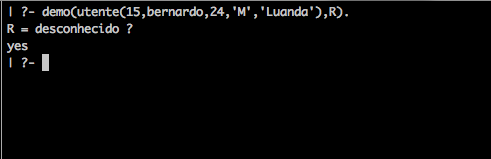
\includegraphics[scale=0.55]{interdito}
\caption{\label{fig:controller}Conhecimento Interdito de um Utente.}
\end{figure}
 
\section{Integridade da Base de Conhecimento}
De forma a manter a integridade da base do conhecimento, e esta esteja de acordo com a realidade que pretendemos representar,é necessário implementar
algum mecanismo que nos garanta isso. Assim, ao longo do trabalho fomos dando uso ao conceito de invariante. Estes permitem-nos controlar em específico a
correta inserção e remoção na Base de Conhecimento. Os invariantes em PROLOG são representados da seguinte forma:
\begin{itemize}
\item +Termo :: Premissas.
\item -Termo :: Premissas.
\end{itemize}
Em Prolog, já existem predicados que nos permitem inserir e remover factos da Base de Conhecimento. Estes são o assert e o retract, respetivamente. No entanto, a utilização destes predicados, exclusivamente, não garante consistência. Sendo assim, é necessário a criação de predicados auxiliares que nos garantam a intregidade da Base de Conhecimento.
Portanto para a realização da evolução deve ser garantido que não exista conhecimento positivo,negativo e imperfeito sendo que este último é definido a custa de exceções. Com base nisso os invariantes adotados tornaram-se muito semelhantes e obedecem o seguinte padrão:
\begin{lstlisting}

+prestador(IdPrestador,IdServ,Nome,Idade,Sexo) :: (
  integer(IdPrestador),
  validaSexo(Sexo),
  Idade>=0,
  findall(IdPrestador,prestador(IdPrestador,_,_,_,_),S1),
    findall(IdPrestador,-prestador(IdPrestador,_,_,_,_),S2),
    findall(IdPrestador,excecao(prestador(IdPrestador,_,_,_,_)),S3),
    length(S1,N1),
    length(S2,N2),
    length(S3,N3),
    N is N1+N2+N3,
  N=<1).

-prestador(IdPrestador,IdServ,Nome,Idade,Sexo) :: (
  findall(IdConsult,prestador(IdPrestador,_,_,_,_),S1),
  length(S1,N),
  N==0).

+(-prestador(IdPrestador,IdServ,Nome,Idade,Sexo))::(
  findall(IdPrestador,prestador(IdPrestador,_,_,_,_),S1),
    findall(IdPrestador,-prestador(IdPrestador,_,_,_,_),S2),
    findall(IdPrestador,excecao(prestador(IdPrestador,_,_,_,_)),S3),
    length(S1,N1),
    length(S2,N2),
    length(S3,N3),
    N is N1+N2+N3,
  N=<1).

\end{lstlisting}
Sendo que para os restantes basta uma alteração para o respectivo predicado e os respectivos átomos.


\subsection{Inserção de Conhecimento}
Como já havia sido dito anteriormente o uso exclusivo da função assert não garante a integridade, para tal surgiu um conjunto de condições que são
verificadas de modo a presevar a consistência da base de conhecimento, e só assim inserir conhecimento. Este processo foi denominado por evolução.
É Implementado do seguinte modo:
\begin{lstlisting}
evolucao(T) :-
findall( I,+T::I,Li ),
insercao( T ),
teste( Li ).

insercao(T) :- assert(T).
insercao(T) :- retract(T), !, fail.
\end{lstlisting}

Sendo que agora existe a necessidade de lidarmos com o conhecimento negativo surgiu a necessidade de criar uma função que lidasse
com a evolução deste conhecimento, tendo sido ela implementada da seguinte maneira:
\begin{lstlisting}
evolucaoNeg(T) :- findall(I,+(-T)::I,Li),
                  teste(Li),
                  assert(-T).
\end{lstlisting}

\subsection{Remoção de conhecimento}

Para a remoção do conhecimento o processo foi análogo ao de inserção, só que para este caso concreto o uso exclusivo do retract não garante a integridade, para tal surgiu um conjunto de condições de modo a preservar a consistência da base de conhecimento, e só assim remover conhecimento.
Este processo foi denominado por involução.É implementado do seguinte modo:

\begin{lstlisting}
involucao(T) :- T,
findall(I,-T::I,Li),
remocao(T),
teste(Li).

remocao(T) :- retract(T).
remocao(T) :- assert(T), !, fail.
\end{lstlisting}

Sendo que agora existe a necessidade de lidarmos com o conhecimento negativo surgiu a necessidade de criar uma função que lidasse
com a evolução deste conhecimento, tendo sido ela implementada da seguinte maneira:

\begin{lstlisting}
involucaoNeg(T) :- findall(I,+(-T)::I,Li),
                   teste(Li),
                   retract(-T).   
\end{lstlisting}



\subsection{Conhecimento Incerto}

Para lidar com o conhecimento incerto optou-se por seguir dois processos distintos:\newline

1º Inserir conhecimento incerto sem ser repetido, tendo sido tirado partido da seguinte função:
\begin{lstlisting}
evolucaoNameIncerto(utente(IdUt,Nome,Idade,Sexo,Cidade)) :-
        evolucao(utente(IdUt,Nome,Idade,Sexo,Cidade)),
        assert(((excecao(utente(Id,N,I,S,C))) :- utente(Id,Nome,I,S,C))),
        assert(uncertaintyName(Nome)).
\end{lstlisting}

A imagem a seguir, retrata a tentativa de inserir um conhecimento incerto já existente e um conhecimento incerto
novo, sendo o primeiro caso rejeitado face a existência do mesmo.

\begin{figure}[H]
\centering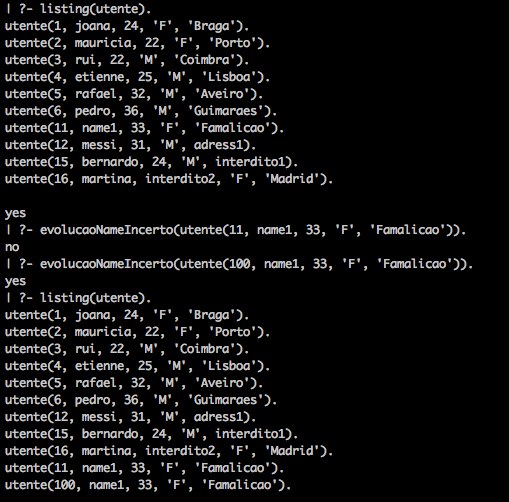
\includegraphics[scale=0.55]{eincerto}
\caption{\label{fig:controller} Evolução do conhecimento Incerto.}
\end{figure}

2º Modificação de conhecimento incerto para Conhecimento Perfeito:

Para este caso em concreto optou-se por corrigir o conhecimento incerto partindo do princípio que o novo valor a ser inserido
fosse o correto,e para a realização desta etapa criou-se por exemplo o seguinte predicado:

\begin{lstlisting}
evolucaoAdressPerfeito(utente(IdUt,Nome,Idade,Sexo,Cidade)) :-
              nao(existeAdressIncerto(utente(IdUt,Nome,Idade,Sexo,Cidade))),
              existeAdressIncerto2(utente(IdUt,Nome,Idade,Sexo,Cidade),L),
              involucaoAdressIncerto(utente(IdUt,Nome,Idade,Sexo,L)),
              evolucao(utente(IdUt,Nome,Idade,Sexo,Cidade)). 
\end{lstlisting}

A imagem a seguir, retrata a evolução de um conhecimento incerto para conhecimento perfeito.

\begin{figure}[H]
\centering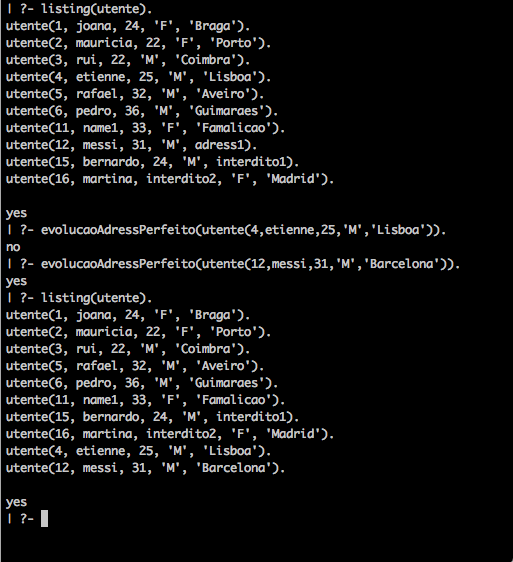
\includegraphics[scale=0.55]{pincerto}
\caption{\label{fig:controller} Evolução do conhecimento Incerto.}
\end{figure}


\subsection{Conhecimento Impreciso}

Relativamente ao conhecimento impreciso decidiu-se fazer modificações ao conhecimento incerto encontrado de modo a ter-se uma transição entre conhecimentos na nossa base de conhecimento, isto é, puder sair de um conhecimento do tipo incerto para algo do tipo impreciso, embora que qualquer interrogação feita sobre o mesmo o resultado será idêntico.
Para implementar esta funcionalidade tirou-se partido de funções que posteriormente seram anexadas.

Optou-se por uma questão de simplificação que o conhecimento impreciso a ser evoluído seria extraído de um conjunto de valores, e ser evoluído recursivamente.

\begin{figure}[H]
\centering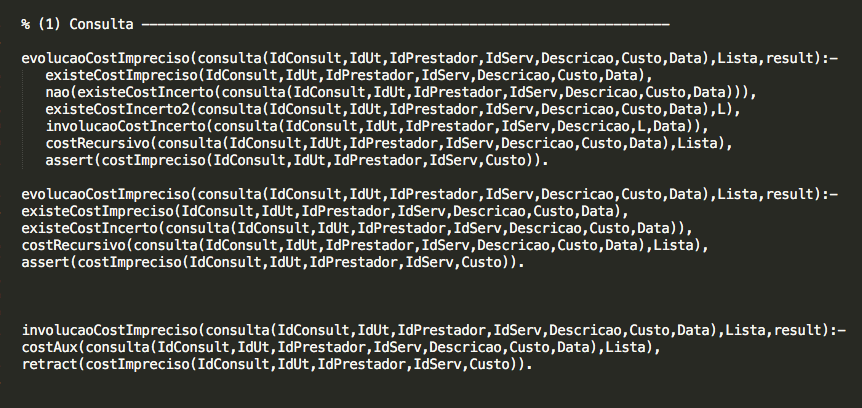
\includegraphics[scale=0.55]{evolucaoConsulta}
\caption{\label{fig:controller} Evolução do conhecimento Impreciso.}
\end{figure}

A imagem a seguir demostra a utilização do código apresentado e os resultados esperados.

\begin{figure}[H]
\centering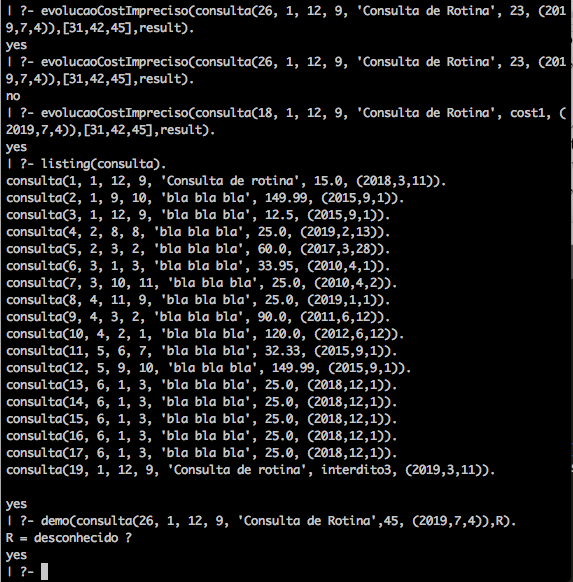
\includegraphics[scale=0.55]{imprecisooo}
\caption{\label{fig:controller} Evolução do conhecimento Impreciso.}
\end{figure}


\subsection{Conhecimento Interdito}

Relativamente ao conhecimento interdito , este só deve ser inserido e nunca modificado sendo que para isso bastou 
inserir a respectiva exceção bem como o seu invariante.

\begin{figure}[H]
\centering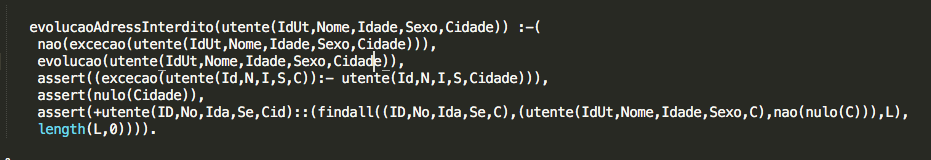
\includegraphics[scale=0.55]{adressInter}
\caption{\label{fig:controller} Evolução do conhecimento Interdito.}
\end{figure}


\begin{figure}[H]
\centering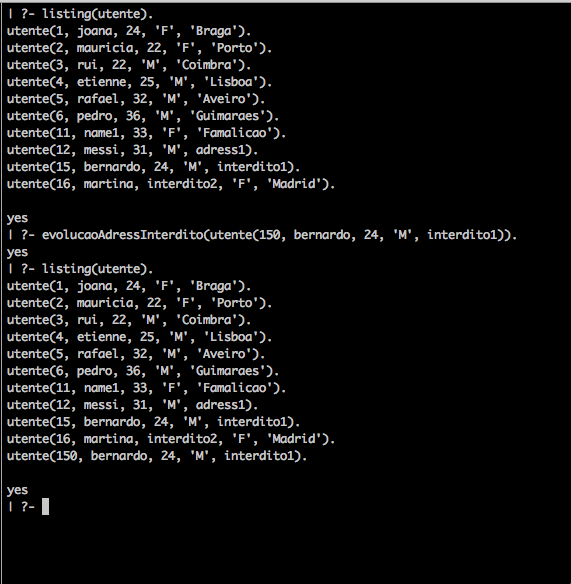
\includegraphics[scale=0.55]{interditooo}
\caption{\label{fig:controller} Evolução do conhecimento Interdito.}
\end{figure}

\section{Sistema de Inferência}

Foi desenvolvido um sistema que permite implementar mecanismos de inferência sobre três tipos de valores nulos, que concretizam situações de informação incompleta. Este sistema suporta três respostas possíveis:
\begin{itemize}
\item verdadeiro.
\item falso.
\item desconhecido.
\end{itemize}

Para tal foi desenvolvido o predicado demo que por sua vez recebe dois argumentos, sendo um deles à Questão a ser colocada  e o segundo a 
Resposta da questão colocada.

\begin{lstlisting}
demo( Questao,verdadeiro):-Questao.
demo(Questao,falso):- -Questao.
demo(Questao,desconhecido):-
                  nao(Questao),
                  nao(-Questao).
\end{lstlisting}

Sendo que esse predicado apresenta limitações no que concerne a quantidade de questões decidiu-se abrangir as conjunções e disjunções ao nosso demonstrador e por fim gerar uma espécie de map do demonstrador podendo assim operar sobre um conjunto de questões.\newline
De seguida são representadas todas as combinações possíveis das conjunções e disjunções bem como as cláusulas que as representam:\newline

\textbf{Disjunção:}
\begin{lstlisting}
demo(Q1, ou, Q2, F) :- demo(Q1, F1),
                       demo(Q2, F2),
                       disjuncao(F1, F2, F).


\end{lstlisting}


\begin{center}
 \begin{tabular}{||c c c c||} 
 \hline
 Questão1 & Questão2 & Resposta \\ [0.5ex] 
 \hline\hline
 Verdadeiro & Verdadeiro & Verdadeiro \\ 
 \hline
 Verdadeiro & Falso & Verdadeiro \\
 \hline
 Verdadeiro & Desconhecido & Verdadeiro\\
 \hline
  Falso & Falso & Falso \\
 \hline
  Falso & Verdadeiro & Verdadeiro \\
 \hline
  Falso & Desconhecido & Desconhecido \\
 \hline
  Desconhecido & Desconhecido & Desconhecido \\
 \hline
  Desconhecido & Verdadeiro & Verdadeiro \\
 \hline
  Desconhecido & Falso & Desconhecido \\ [1ex] 
 \hline
\end{tabular}
\end{center}


\textbf{Conjunção:}
\begin{lstlisting}
demo(Q1, e, Q2, F) :- demo(Q1, F1),
                    demo(Q2, F2),
                    conjuncao(F1, F2, F).


\end{lstlisting}

\begin{center}
\begin{tabular}{||c c c c||} 
\hline
Questão1 & Questão2 & Resposta \\ [0.5ex] 
 \hline\hline
 Verdadeiro & Verdadeiro & Verdadeiro \\ 
 \hline
 Verdadeiro & Falso & Falso \\
 \hline
 Verdadeiro & Desconhecido & Desconhecido\\
 \hline
  Falso & Falso & Falso \\
 \hline
  Falso & Verdadeiro & Falso \\
 \hline
  Falso & Desconhecido & Falso \\
 \hline
  Desconhecido & Desconhecido & Desconhecido \\
 \hline
  Desconhecido & Verdadeiro & Desconhecido \\
 \hline
  Desconhecido & Falso & Falso \\ [1ex] 
 \hline
\end{tabular} 
\end{center}

\textbf{DemoMap:}

O demoMap recebe dois argumentos, uma lista de questões e uma lista de respostas para as questões passadas como parâmetro, foi implementado de 
modo a ser possível serem respondidas várias questões em simultâneo.
\begin{lstlisting}
demoMap([], []).
demoMap([X|L], [R|S]) :- demo(X, R),
                          demoMap(L, S).
\end{lstlisting}
\begin{figure}[H]
\centering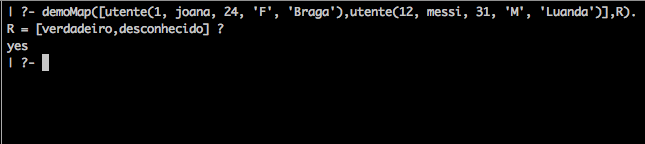
\includegraphics[scale=0.55]{demoMap}
\caption{\label{fig:controller}Map Demo.}
\end{figure}

\section{Conclusão}

A realização deste trabalho prático permitiu consolidar o conhecimento adquirido ao longo das aulas, no que concerne
à programação em lógica estendida e conhecimento imperfeito. Como tal, o suporte utilizado para caracterizar um universo de discurso na área da prestação de cuidados de saúde foi o PROLOG.
Em forma de conclusão, o grupo considera que conseguiu corresponder as expectativas  e consolidar os conceitos relativos ao conhecimento
imperfeito e às variantes que este apresenta. 
Sendo que uma das principais dificuldades encontradas no desenvolvimento deste sistema passou pela forma como era feita a evolução de conhecimentos face aos diferentes tipo de conhecimento, sendo assim no que concerne a melhorias , passa por num futuro próximo inserir outros factos de modo a aproximar o trabalho de um contexto mais real, factos esses como receitas médicas e medicamentos.
\newpage
\section{Referências Bibliográficas}


\begin{thebibliography}{9}
\bibitem{latexcompanion} 
Cesar Analide, Jose Neves. 
\textit{"Representação de Informação Incompleta"}. 

 
\bibitem{einstein} 
Ivan Bratko. 
\textit{"PROLOG: Programming for Artificial Intelligence"}. 

\end{thebibliography}




\newpage

\section{Funções Auxiliares}
\begin{lstlisting}
%---------------------------------------------------------------------------------


demo( Questao,verdadeiro):-Questao.

demo(Questao,falso):- -Questao.

demo(Questao,desconhecido):-nao(Questao),
                  nao(-Questao).

%--------------------------------- - - - - - - - - - -  -  -  -  -   -


demo(Q1, ou, Q2, F) :- demo(Q1, F1),
                     demo(Q2, F2),
                     disjuncao(F1, F2, F).

demo(Q1, e, Q2, F) :- demo(Q1, F1),
                    demo(Q2, F2),
                    conjuncao(F1, F2, F).

%--------------------------------- - - - - - - - - - -  -  -  -  -   -


disjuncao(verdadeiro, X, verdadeiro).
disjuncao(X, verdadeiro, verdadeiro).
disjuncao(desconhecido, Y, desconhecido) :- Y \= verdadeiro.
disjuncao(Y, desconhecido, desconhecido) :- Y \= verdadeiro.
disjuncao(falso, falso, falso).


%--------------------------------- - - - - - - - - - -  -  -  -  -   -


conjuncao(verdadeiro, verdadeiro, verdadeiro).
conjuncao(falso, _, falso).
conjuncao(_, falso, falso).
conjuncao(desconhecido, verdadeiro, desconhecido).
conjuncao(verdadeiro, desconhecido, desconhecido).

%--------------------------------- - - - - - - - - - -  -  -  -  -   -


demoMap([], []).
demoMap([X|L], [R|S]) :- demo(X, R),
                          demoMap(L, S).

%--------------------------------------------------------------------------------------------
nao(T) :- T, !, fail.
nao(T).
%--------------------------------------------------------------------------------------------
teste([]).
teste([I|Is]):-I,teste(Is).


insercao(T) :- assert(T).
insercao(T) :- retract(T), !, fail.


remocao(T) :- retract(T).
remocao(T) :- assert(T), !, fail.


evolucao(T) :-  findall(I,+T::I,Li),
                insercao(T),
                teste(Li).

involucao(T) :- T,
                findall(I,-T::I,Li),
                remocao(T),
                teste(Li).

evolucaoNeg(T) :- findall(I,+(-T)::I,Li),
                  teste(Li),
                  assert(-T).

involucaoNeg(T) :- findall(I,+(-T)::I,Li),
                   teste(Li),
                   retract(-T).     

%-----------------PREDICADOS AUXILIARES---------------------------------------------------------------------------

existeAdressIncerto(utente(IdUt,Nome,Idade,Sexo,Cidade)) :- 
(findall(City,(utente(IdUt,N,I,S, City),uncertaintyAdress(City)),L),
length(L,0)).
                                                              

existeAdressIncerto2(utente(IdUt,Nome,Idade,Sexo,Cidade),L) :- 
(findall( (City), (utente(IdUt,N,I,S, City),uncertaintyAdress(City)),[L|Ls])).

%-----------------------------------------------------------------------------------------------------------------

existeNameIncerto(utente(IdUt,Nome,Idade,Sexo,Cidade)) :- 
(findall(Name,(utente(IdUt,Name,I,S,C),uncertaintyName(Name)),L),
length(L,0)).
                                                              

existeNameIncerto2(utente(IdUt,Nome,Idade,Sexo,Cidade),L) :- 
(findall( (Name), (utente(IdUt,Name,I,S,C),uncertaintyName(Name)),[L|Ls])).

%-----------------------------------------------------------------------------------------------------------------


existeInstitutionIncerto(servico(IdServ,Especialidade,Instituicao,Cidade)) :- 
(findall(Insti,(servico(IdServ,E,Insti,C),uncertaintyInstitution(Insti)),L),
length(L,0)).
                                                               

existeInstitutionIncerto2(servico(IdServ,Especialidade,Instituicao,Cidade),L) :- 
(findall((Insti),(servico(IdServ,E,Insti,C),uncertaintyInstitution(Insti)),[L|Ls])).

%-----------------------------------------------------------------------------------------------------------------
existeCostIncerto(consulta(IdConsult,IdUt,IdPrestador,IdServ,Descricao,Custo,Data)) :- 
(findall(Cost,(consulta(IdConsult,IdUt,IdPrestador,IdServ,D,Cost,Da), uncertaintyCost(Cost)),L ),
length(L,0)).

existeCostIncerto2(consulta(IdConsult,IdUt,IdPrestador,IdServ,Descricao,Custo,Data), L) :- 
(findall( (Cost), (consulta(IdConsult,IdUt,IdPrestador,IdServ,D,Cost,Da), uncertaintyCost(Cost)),[L|Ls])).
                                                                 

existeCostImpreciso(IdConsult,IdUt,IdPrestador,IdServ,Descricao,Custo,Data):-
(findall((Idc,Idu,Idp,Ids),(costImpreciso(IdConsult,IdUt,IdPrestador,IdServ,Custo)),L),
length(L,0)).
%-----------------------------------------------------------------------------------------------------------------
costRecursivo(consulta(IdConsult,IdUt,IdPrestador,IdServ,Descricao,Custo,Data),[Head|[]]) :- 
evolucao(excecao(consulta(IdConsult,IdUt,IdPrestador,IdServ,Descricao,Head,Data))).

costRecursivo(consulta(IdConsult,IdUt,IdPrestador,IdServ,Descricao,Custo,Data),[Head|Tail]) :- 
evolucao(excecao(consulta(IdConsult,IdUt,IdPrestador,IdServ,Descricao,Head,Data))),
costRecursivo(consulta(IdConsult,IdUt,IdPrestador,IdServ,Descricao,Custo,Data),Tail).


costAux(consulta(IdConsult,IdUt,IdPrestador,IdServ,Descricao,Custo,Data),[Head|[]]) :- 
involucao(excecao(consulta(IdConsult,IdUt,IdPrestador,IdServ,Descricao,Head,Data))).

costAux(consulta(IdConsult,IdUt,IdPrestador,IdServ,Descricao,Custo,Data),[Head|Tail]) :- 
involucao(excecao(consulta(IdConsult,IdUt,IdPrestador,IdServ,Descricao,Head,Data))),
costAux(consulta(IdConsult,IdUt,IdPrestador,IdServ,Descricao,Custo,Data),Tail).

--------------------------------------------------------------------

\end{lstlisting}
\end{document}
